\beforesec
\section{Results} 
\label{sec:results}
\postsec

This section presents our key experimental findings.
First, we show that WiSE-FT boosts the accuracy of a fine-tuned CLIP model on five ImageNet distribution shifts studied by \citet{radford2021learning}, while maintaining or improving ImageNet accuracy.
Next, we present additional experiments, including more distribution shifts, the effect of hyperparameters, accuracy improvements on the reference distribution, and experiments in the low-data regime. 
Finally, we demonstrate that our findings are more broadly applicable by exploring WiSE-FT for BASIC \cite{pham2021scaling}, ALIGN \cite{jia2021scaling}, and a ViT-H/14 \cite{dosovitskiy2021an} model pre-trained on JFT-300M \cite{sun2017revisiting}.

\begin{table*}
\setlength\tabcolsep{5.1pt}
\small
\begin{center}
\begin{tabular}{lc|ccccc|cc}
\toprule
{} &            &             \multicolumn{5}{c|}{Distribution shifts}             &                    Avg &                        Avg\\
{} &           IN (reference) &             IN-V2 &              IN-R &                 IN-Sketch &                 ObjectNet* &              IN-A &                    shifts &                        ref., shifts\\
\midrule
CLIP \texttt{ViT-L/14@336px} & & & & & & & &\\
\quad Zero-shot \cite{radford2021learning} &                    76.2 &                    70.1 &                    88.9 &                             60.2 &                             70.0 &                    77.2 &                             73.3 &                             74.8 \\
\quad  Fine-tuned LC \cite{radford2021learning} &                    85.4 &                    75.9 &                    84.2 &                             57.4 &                             66.2 &                    75.3 &                             71.8 &                             78.6 \\
\quad  Zero-shot (PyTorch)                   &                    76.6 &                    70.5 &                    89.0 &                             60.9 &                             69.1 &                    77.7 &                             73.4 &                             75.0 \\
\quad  Fine-tuned LC (ours)              &                    85.2 &                    75.8 &                    85.3 &                             58.7 &                             67.2 &                    76.1 &                             72.6 &                             78.9 \\
\quad  Fine-tuned E2E (ours)                     &                    86.2 &                    76.8 &                    79.8 &                             57.9 &                             63.3 &                    65.4 &                             68.6 &                             77.4 \\\midrule
\quad  WiSE-FT (ours) & & & & & & & &\\
\quad \quad LC, $\alpha{=}0.5$     &                    83.7 &                    76.3 &                    89.6 &  63.0 &  70.7 &  79.7 &  75.9 &  79.8 \\
\quad \quad LC, optimal $\alpha$        &                    85.3 &                    76.9 &                    89.8 &                             63.0 &                             70.7 &                    79.7 &                             75.9 &                             80.2 \\
\quad \quad E2E, $\alpha{=}0.5$ &                    86.8 &  \textbf{79.5} &                    89.4 &                    64.7 &                    71.1 &                    79.9 &                    76.9 &                    81.8 \\

\quad \quad E2E, optimal $\alpha$       &  \textbf{87.1} &  \textbf{79.5} &  \textbf{90.3} &  \textbf{65.0} &  \textbf{72.1} &  \textbf{81.0} & \textbf{77.4} &  \textbf{81.9} \\


\bottomrule
\end{tabular}
\caption{\label{tab:main} Accuracy of various methods on ImageNet and derived distribution shifts for CLIP \texttt{ViT-L/14@336px} \cite{radford2021learning}. E2E: end-to-end; LC: linear classifier. \textit{Avg shifts} displays the mean performance among the five distribution shifts, while \textit{Avg reference, shifts} shows the average of ImageNet (reference) and Avg shifts. For optimal $\alpha$, we choose the single mixing coefficient that maximizes the column. Results for additional models are provided in Appendix~\ref{sec:more-models}.
}

\end{center}
\end{table*}









\paragraph{Main results: ImageNet and associated distribution shifts.}
\label{sec:main_results}
As illustrated in Figure~\ref{fig:fig1}, when the \ALPHA{} $\alpha$ varies from $0$ to $1$, $\mathsf{wse}(\cdot, \alpha)$ is able to simultaneously improve accuracy on both the reference and shifted distributions. A breakdown for each dataset is shown in Appendix~\ref{sec:fig1breakdown}. 
Table \ref{tab:main} presents our main results on ImageNet and five derived distribution shifts. 
WiSE-FT (end-to-end, $\alpha{=}0.5$) outperforms numerous strong models in both average accuracy under distribution shift and the average accuracy on the reference and shifted distributions.
While future work may lead to more sophisticated strategies for choosing the mixing coefficient $\alpha$, $\alpha{=}0.5$ yields close to optimal performance across a range of experiments. Hence, we recommend $\alpha{=}0.5$ when no domain knowledge is available. Appendix \ref{sec:appendix_alpha} further explores the effect of $\alpha$. Moreover, results for twelve additional backbones are shown in Appendix \ref{sec:appendix_additional_exps}. 


\paragraph{Robustness on additional distribution shifts.}
Beyond the five distribution shifts derived from ImageNet, WiSE-FT consistently improves robustness on a diverse set of further distributions shifts including geographic shifts in satellite imagery and  wildlife recognition (WILDS-FMoW \cite{wilds2021, christie2018functional}, WILDS-iWildCam \cite{wilds2021, beery2021iwildcam}), reproductions of the popular image classification dataset CIFAR-10 \cite{krizhevsky2009learning} with a distribution shift (CIFAR-10.1 \cite{pmlr-v97-recht19a} and CIFAR-10.2 \cite{lu2020harder}), and datasets with distribution shift induced by temporal perturbations in videos (ImageNet-Vid-Robust and YTBB-Robust \cite{shankar2020evaluating}). 
Concretely, WiSE-FT ($\alpha{=}0.5$) improves performance under distribution shift by 3.5, 6.2, 1.7, 2.1, 9.0 and 23.2 pp relative to the fine-tuned solution while decreasing performance on the reference distribution by at most 0.3 pp (accuracy on the reference distribution often improves).
In contrast to the ImageNet distribution shifts, the zero-shot model initially achieves less than 30\% accuracy on the WILDS distribution shifts, and WiSE-FT provides improvements regardless.
Appendix \ref{sec:moreshift} (Figure~\ref{fig:fig_more_shifts} and Table~\ref{tab:moreshifts}) includes more detailed results.

\begin{figure}
    \centering
    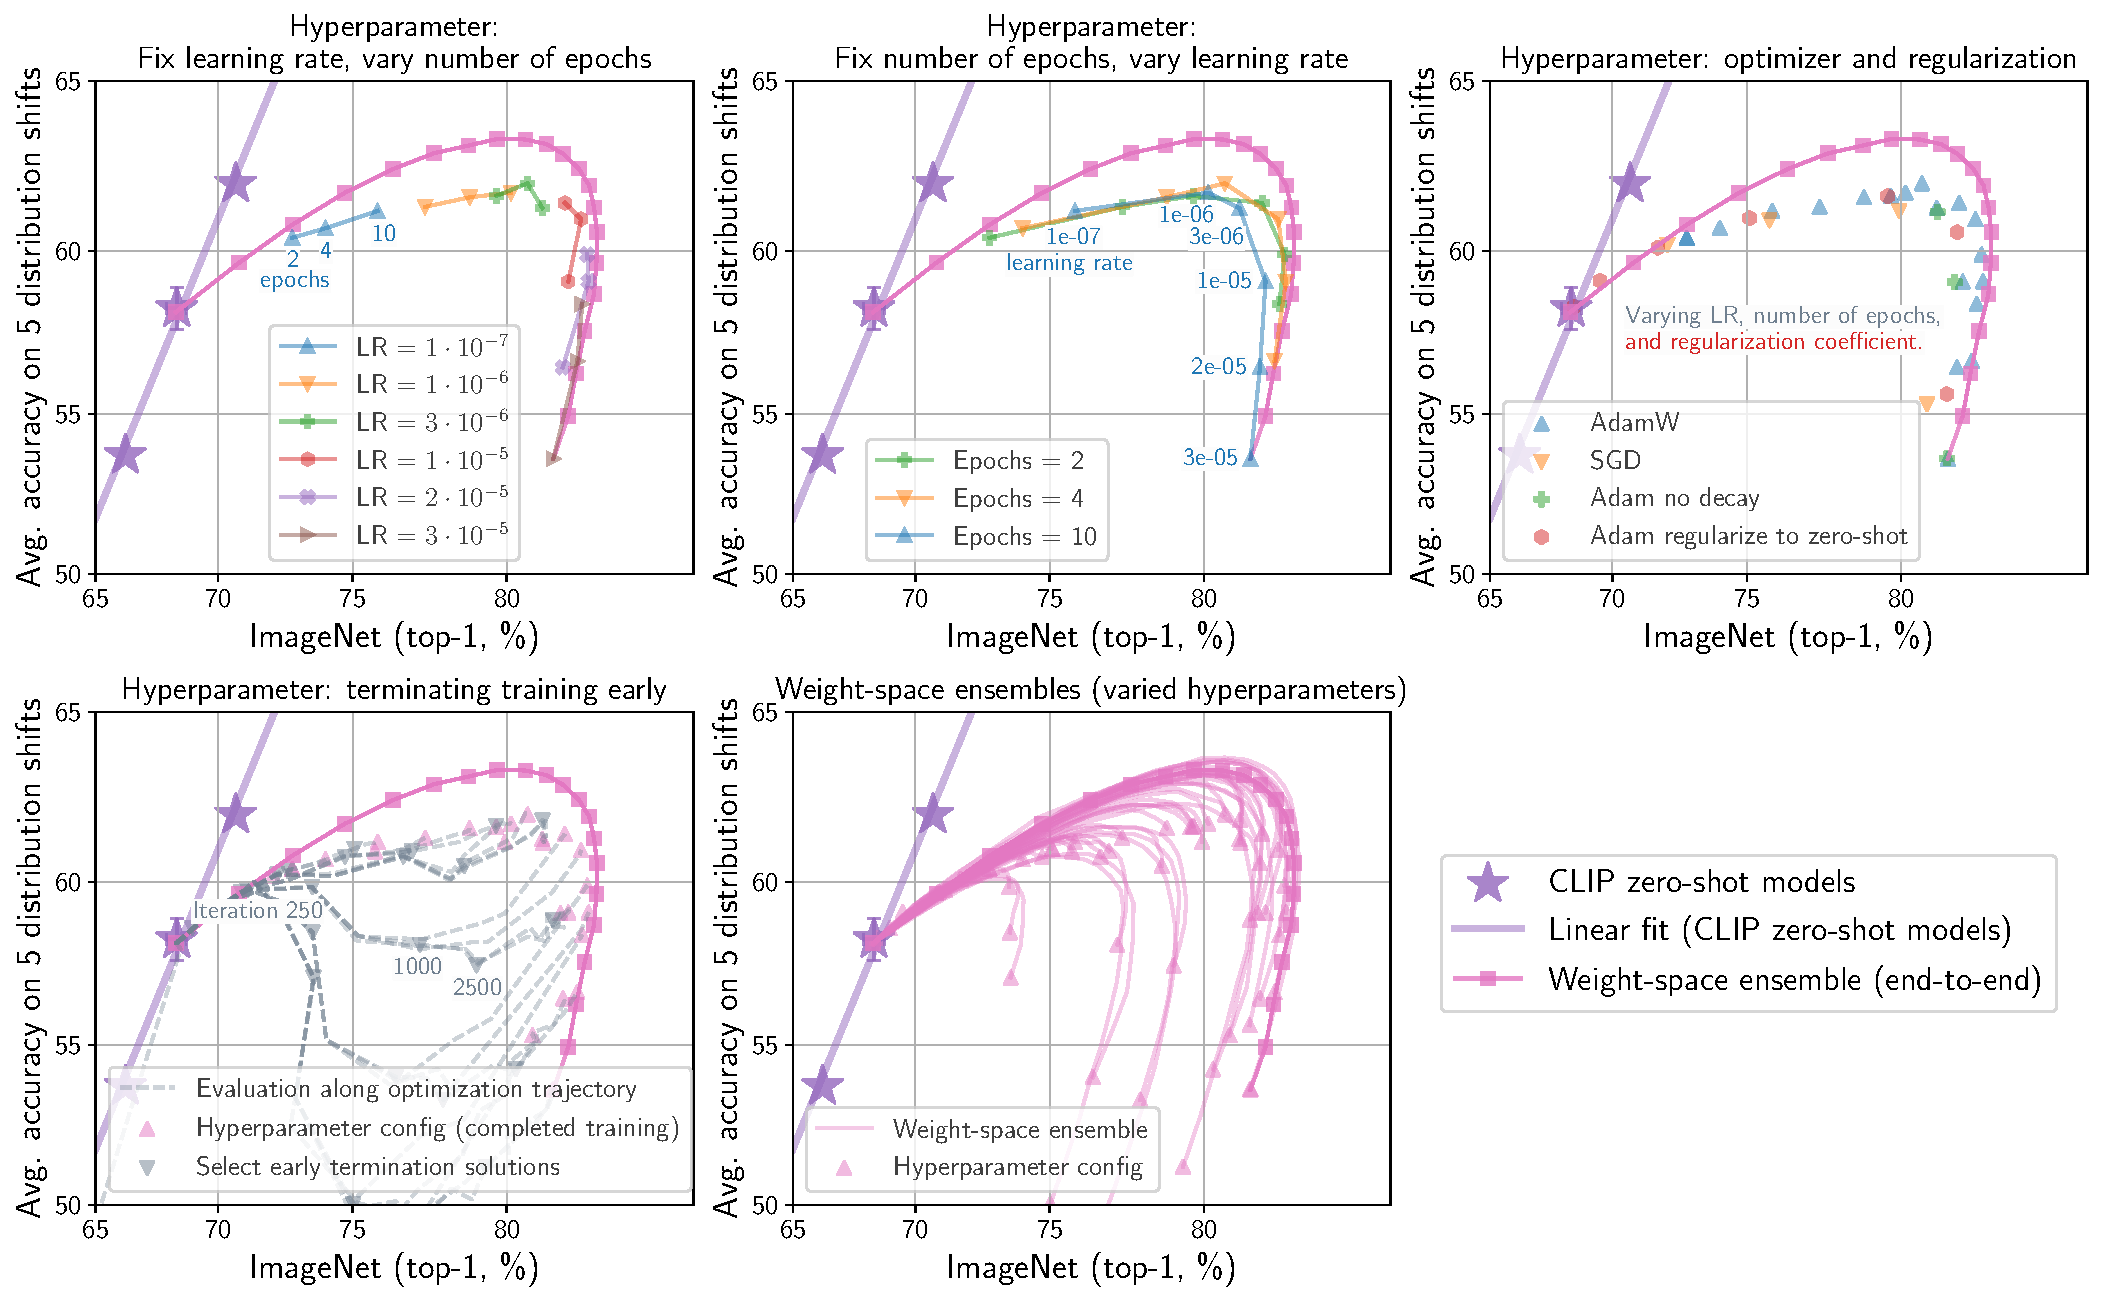
\includegraphics[width=\textwidth]{figures/more_hparams.pdf}
    \caption{
    The robustness of fine-tuned models varies substantially under even small changes in hyperparameters.
    Applying WiSE-FT addresses this brittleness and can remove the trade-off between accuracy on the reference and shifted distributions.
    Results shown for CLIP \texttt{ViT-B/16} fine-tuned with cosine-annealing learning rate schedule and all models in the top left and top middle plots are fine-tuned with AdamW \cite{loshchilov2018decoupled}. Moreover, 
    \textit{regularize to zero-shot} appends the regularizer $\lambda \mleft\|\theta - \theta_0  \mright\|_2^2$ to the fine-tuning objective, where $\theta_0$ are the parameters of the zero-shot model.
    }
    \label{fig:hparams}
\end{figure}

\paragraph{Hyperparameter variation and alternatives.} As illustrated by Figure~\ref{fig:hparams}, moderate changes in standard hyperparameters such as the learning rate or the number of epochs can substantially affect performance under distribution shift. Moreover, these performance differences cannot be detected reliably from model performance on reference data alone.
For instance, while training for 10 epochs with learning rate $3 \cdot 10^{-5}$ and $3 \cdot 10^{-6}$ lead to a small accuracy difference on ImageNet (0.3 pp), accuracy under distribution shift varies by as much as 8 pp.

Furthermore, tuning hyperparameters on ImageNet data can also reduce robustness. For instance, while moving from small to moderate learning rates ($10^{-7}$ to $3 \cdot 10^{-5}$) improves performance on ImageNet by 5 pp, it also deteriorates accuracy under distribution shift by 8 pp.

WiSE-FT addresses this brittleness of hyperparameter tuning: even when using a learning rate $3 \cdot 10^{-5}$ where standard fine-tuning leads to low robustness, applying WiSE-FT removes the trade-off between accuracy on the reference and shifted distributions. 
The models which can be achieved by varying $\alpha$ are as good or better than those achievable by other hyperparameter configurations. Then, instead of searching over a wide range of hyperparameters, only $\alpha$ needs to be considered. Moreover, evaluating different values of $\alpha$ does not require training new models.

There is no hyperparameter in Figure~\ref{fig:hparams} which can be varied to match or exceed the optimal curve produced by WiSE-FT.
In our experiments, this frontier is reached only through methods that average model weights, either using WiSE-FT or
with a more sophisticated averaging scheme: keeping an exponential moving average of all model iterates (EMA, \cite{szegedy2016rethinking}).
Comparisons with EMA are detailed in Appendix~\ref{sec:ema}.

\customfootnotetext{$*$}{Although this table considers ImageNet class names, ObjectNet provides alternative class names which can improve the performance of zero-shot CLIP by 2.3 percentage points (Appendix \ref{sec:objectnet}).}

Additional comparisons are also presented in Appendix~\ref{sec:baselines-appendix}, including distillation, additional regularization, and CoOp \cite{coop}. Finally, Appendix~\ref{sec:dataaug} recreates Figure~\ref{fig:hparams} with stronger data augmentation and finds similar trends.







\paragraph{Accuracy gains on reference distributions.}
Beyond robustness to distribution shift, Table \ref{tab:id_gains} demonstrates that WiSE-FT also improves accuracy after fine-tuning on seven datasets. When fine-tuning end-to-end on ImageNet, CIFAR-10, CIFAR-100, Describable Textures, Food-101, SUN397, and Stanford Cars, WiSE-FT reduces relative error by 4 to 49\%.
Even though standard fine-tuning directly optimizes for high accuracy on the reference distribution, WiSE-FT achieves better performance.
Appendix \ref{sec:low-data} includes more details, including explorations in the low-data regime.






\begin{table}
\setlength\tabcolsep{3.5pt}
\begin{center}
\small
\begin{tabular}{l@{\hskip .2in}c@{\hskip .2in}ccccccc}
\toprule
{} &     ImageNet &      CIFAR10 &     CIFAR100 &         Cars &          DTD &       SUN397 &      Food101 \\          \midrule                                                                             Standard fine-tuning    &         86.2 &                                            98.6 &                                            92.2 &                                            91.6 &                                            81.9 &                                            80.7 &                                            94.4 \\                   WiSE-FT ($\alpha{=}0.5$) &  86.8 {\scriptsize\textcolor{LimeGreen}{(+0.6)}} &  99.3 {\scriptsize\textcolor{LimeGreen}{(+0.7)}} &  93.3 {\scriptsize\textcolor{LimeGreen}{(+1.1)}} &  93.3 {\scriptsize\textcolor{LimeGreen}{(+1.7)}} &  84.6 {\scriptsize\textcolor{LimeGreen}{(+2.8)}} &  83.2 {\scriptsize\textcolor{LimeGreen}{(+2.5)}} &  96.1 {\scriptsize\textcolor{LimeGreen}{(+1.6)}} \\                                                         WiSE-FT (opt. $\alpha$)  &  87.1 {\scriptsize\textcolor{LimeGreen}{(+0.9)}} &  99.5 {\scriptsize\textcolor{LimeGreen}{(+0.8)}} &  93.4 {\scriptsize\textcolor{LimeGreen}{(+1.2)}} &  93.6 {\scriptsize\textcolor{LimeGreen}{(+2.0)}} &  85.2 {\scriptsize\textcolor{LimeGreen}{(+3.3)}} &  83.3 {\scriptsize\textcolor{LimeGreen}{(+2.6)}} &  96.2 {\scriptsize\textcolor{LimeGreen}{(+1.8)}} \\  
\bottomrule
\end{tabular}
\caption{\label{tab:id_gains} Beyond robustness, WiSE-FT can improve accuracy after fine-tuning on several datasets.}%
\end{center}
\end{table}


\paragraph{Beyond CLIP.} Figure~\ref{fig:beyondclip} illustrates that WiSE-FT is generally applicable to zero-shot models beyond CLIP, and beyond models pre-trained contrastively with image-text pairs. First, we interpolate between the weights of the zero-shot and fine-tuned BASIC-L model \cite{pham2021scaling}, finding that $\alpha{=}0.5$ improves average accuracy on five distribution shifts derived from ImageNet by over 7 pp while improving ImageNet accuracy by 0.4 pp relative to the fine-tuned BASIC-L model (a per-dataset breakdown is provided in Figure~\ref{fig:basicbreakdown} and Table~\ref{tab:basic_l} of the Appendix).
As in \citet{pham2021scaling}, the model is fine-tuned using a contrastive loss and half of the ImageNet training data. 
WiSE-FT provides improvements on both reference and shifted distributions, despite these experimental differences.

Next, we consider the application of WiSE-FT to a ViT-H/14 model \cite{dosovitskiy2021an} pre-trained on JFT-300M \cite{sun2017revisiting},
where the zero-shot classifier is constructed by manually identifying a class correspondence (details provided in Section~\ref{sec:JFT}).
WiSE-FT improves performance under distribution shift over both the zero-shot and fine-tuned models. 
When $\alpha{=}0.8$, WiSE-FT outperforms the fine-tuned model by 2.2 pp on distribution shifts, while maintaining ImageNet performance within 0.2 pp of the fine-tuned model.
This result demonstrates that WiSE-FT can be successfully applied even to models which do not use contrastive image-text pre-training.

Finally, we apply WiSE-FT to the ALIGN model of \citet{jia2021scaling}, which is similar to CLIP but is pre-trained with a different dataset, finding similar trends.


\begin{figure}
    \centering
    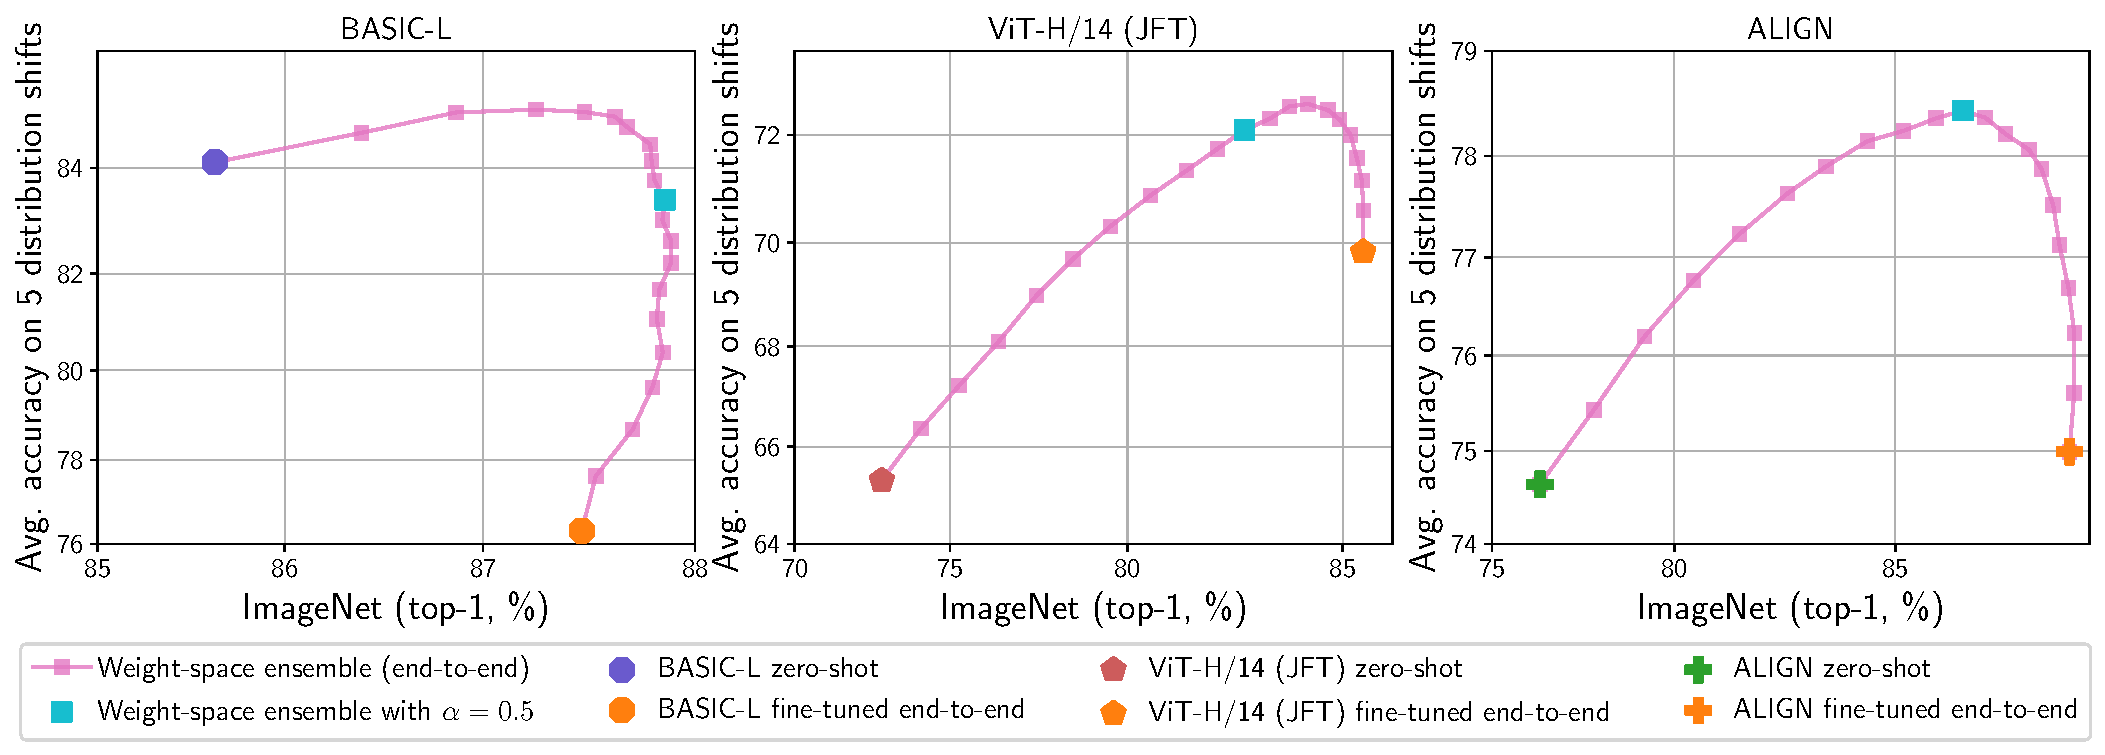
\includegraphics[width=\textwidth]{figures/basic.pdf}
    \caption{WiSE-FT applied to BASIC-L \cite{pham2021scaling}, a ViT-H/14 \cite{dosovitskiy2021an} model pre-trained on JFT-300M \cite{sun2017revisiting} and ALIGN~\cite{jia2021scaling}.}
    \label{fig:beyondclip}
    \vspace*{-0.4cm}
\end{figure}